\documentclass[twocolumn]{article}
\usepackage{amsmath,algorithmic}
\usepackage[dvipdfmx]{graphicx}

%% \setlength{\oddsidemargin}{-0.4mm} 
%% \setlength{\evensidemargin}{\oddsidemargin}
%% \setlength{\textwidth}{170mm} 
\setlength{\textheight}{44\baselineskip}
\addtolength{\textheight}{\topskip}
\setlength{\voffset}{-0.6in}


\bibliographystyle{alpha}

\title{Orthotope Machine}
\author{Takayuki Muranushi}
\begin{document}
\maketitle
\begin{quote}
  In geometry, an orthotope (also called a hyperrectangle or a box) is
  the generalization of a rectangle for higher dimensions, formally
  defined as the Cartesian product of intervals.
\end{quote}

\section{Introduction}

This document describes the {\em Orthotope Machine}, a virtual machine that
operates on multidimensional arrays. The Orthotope Machine is one of the main
components for Paraiso project. The goal of Paraiso project is to create a
high-level programming language for generating massively parallel, explicit
solver algorithms of partial differential equations. 


From computational viewpoint, explicit solvers of partial differential
equations belongs to the algorithm category called stencil codes. Stencil
codes are algorithms that updates the array, each element accessing the nearby
elements in the same pattern (c.f. Fig.\ref{FigureStencilPseudoCode}). Stencil
codes are commonly used algorithms in fields such as solving partial
differential equations and image processing. Code generations and automated
tuning for stencil codes has been studied e.g. \cite{Datta:EECS-2009-177,
  Datta:2008:SCO:1413370.1413375}.

There are many methods other than stencil codes for solving partial
differential equations. They have different merits. A notable project in
progress is Liszt \cite{Chafi:2010:LVH:1932682.1869527}, an embedded DSL in
programmin language Scala, designed for generating hydrodynamics solver on
unstructured mesh.

\begin{figure}
\begin{verbatim}
double a[NY][NX], b[NY][NX];
for (int t=0; t<max_t; ++t) {
  for (int y=1; y<NY-1; ++y) 
    for (int x=1; x<NX-1; ++x) 
      b[y][x] = a[y][x-1] + a[y][x+1] 
              + a[y-1][x] + a[y+1][x];

  for (int y=1; y<NY-1; ++y) 
    for (int x=1; x<NX-1; ++x) 
      a[y][x] += 0.25 * b[y][x];
}
\end{verbatim}
\caption{An example of stencil code.}\label{FigureStencilPseudoCode}
\end{figure}

Many parallel and distributed programming languages has been implemented using
Haskell \cite{CambridgeJournals:114967}. Data Parallel Haskell
\cite{nested-data-parallelism} and
Nepal\cite{springerlink:10.10073-540-44681-8_76} are implementations of NESL,
a language for operating nested arrays.
Accelerate \cite{Chakravarty:2011:AHA:1926354.1926358} and
Nikola \cite{Mainland:2010:NEC:1863523.1863533} are languages to manipulate arrays on GPUs written in Haskell.

We need new languages for parallel hardwares --- this is a long-standing
idea. Many project sought for them, and some failed. Failures from which we
can learn. High Performance Fortran was a very promising approach to introduce
a high-level parallelism in Fortran but, as James Stone told me in Taiwan, and
as is summarised by the project leader
\cite{Kennedy:2007:RFH:1238844.1238851}, it failed.  DEQSOL
\cite{SAGAWANOBUTOSHI:1989-01-15,Kon'no:1986:AIS:324493.325029} was another
project which had design similar to that of Paraiso. The language was
initially designed for Hitachi vector machines. The extension of DEQSOL for
parallel vector machines has been planned \cite{SagawaNobutoshi:1989-03-15}
but seemingly did not realize.

The unique point of Paraiso compared to those projects is its focus on
computational domains that utilize localized access to multidimensional
arrays.

Multidimensional arrays are different from nested arrays. For example in the
psueudocode Fig.\ref{FigureStencilPseudoCode}, in order to calculate {\tt
  b[y][x]} you need to read from {\tt a[y-1][x]} and {\tt a[y+1][x]}, which
are usually located much farther in the memory compared to {\tt a[y][x-32]} or
{\tt a[y][x+64]}. The code generator must be aware of such locality in
multidimensional space.  For most of the cases, the basic equations to be
solved is symmetric under exchange of the axes (X,Y,Z ...). Still, there are
nonnegligible differences between the axes from computational point of view,
especially if the multidimensional arrays are stored in row-major or
column-major order. To utilize the cache and/or vector instructions, we need
to know, or decide upon, the order the array is stored in the memory.

In parallel machines, the array must be decomposed and distributed among
computer nodes. It is important to take care of the continuity in
multidimensional space when making the distribution, so that the
communications cost is lowered. If the data to be communicated is stored
sparsely in the memory, it is a good strategy to gather them manually into a
single buffer and to make a single large communication instead of making lots
of small communications. Due to this gather/scattering cost, not making any
decomposition in one or more directions gives higher performance in some
cases.

The Orthotope Machine is designed to capture and utilize these
characteristics of the multidimensional array computations.

\section{Explicit Solvers of Partial Differential Equations}

\begin{figure*}
\begin{verbatim}
double fluid[NZ][NY][NX];
double flow_x[NZ][NY][NX];
double flow_y[NZ][NY][NX];
double flow_z[NZ][NY][NX];
double dt_local[NZ][NY][NX];

// (1) simulation goes from time t=0 to t=t_max
for (double t=0; t<t_max; t+=dt) {

  // (2) calculate the timescale for each mesh
  for (int z=1; y<NZ-1; ++z) 
    for (int y=1; y<NY-1; ++y) 
      for (int x=1; x<NX-1; ++x) 
        dt_local[z][y][x]=timescale(fluid[z][y][x]);

  // (3) calculate the minimum timescale
  double dt=max_t;
  for (int z=1; y<NZ-1; ++z) 
    for (int y=1; y<NY-1; ++y) 
      for (int x=1; x<NX-1; ++x) 
        dt=min(dt, dt_local[z][y][x]);

  // (4) calculate the flow for each direction
  for (int z=1; y<NZ; ++z) {
    for (int y=1; y<NY; ++y) { 
      for (int x=1; x<NX; ++x) { 
        flow_x[z][y][x]=calc_fx(fluid[z][y][x-1], fluid[z][y][x]);
        flow_y[z][y][x]=calc_fy(fluid[z][y-1][x], fluid[z][y][x]);
        flow_z[z][y][x]=calc_fz(fluid[z-1][y][x], fluid[z][y][x]);
      }
    }
  }

  // (5) move the fluid according to the flow
  for (int z=1; y<NZ-1; ++z) 
    for (int y=1; y<NY-1; ++y) 
      for (int x=1; x<NX-1; ++x)
          fluid[z][y][x] +=
          dt*(flow_x[z][y][x]-flow_x[z][y][x+1])/dx
         +dt*(flow_y[z][y][x]-flow_x[z][y+1][x])/dy
         +dt*(flow_z[z][y][x]-flow_x[z+1][y][x])/dz;

}
\end{verbatim}
\caption{A typical hydrodynamic equations solver does something like
  this.}\label{FigureHydroPseudoCode}
\end{figure*}

Fig. \ref{FigureHydroPseudoCode} shows a pseudocode for a hydrodynamic
equations solver. Although it is a bit simplified from the real solvers, it
shows what components needed to build one.

A common task for the solver is to simulate the evolution of the fluid for a
certain interval of time, say, $0 < t < t_{\mathrm max}$ (1). In the each step
of the simulation, the time {\tt t} increases by a certain amount {\tt dt}.
In many problems, the timestep {\tt dt} is not a constant but depends on the
state of the fluid. In such case, you need to calculate the timesteps adequate
for the fluid state of every mesh (2), and then perform reduction over the entire computational domain to calculate the smallest {\tt dt} (3).


\section{Overall Design of Paraiso, and Orthotope Machine's Role in it}


\section{Definitions of Orthotope, Orthotree, and Distributed Orthotope}

\section{API for Orthotope Machine}


\section{Hardware Model}

\begin{figure*}
  \begin{center}
    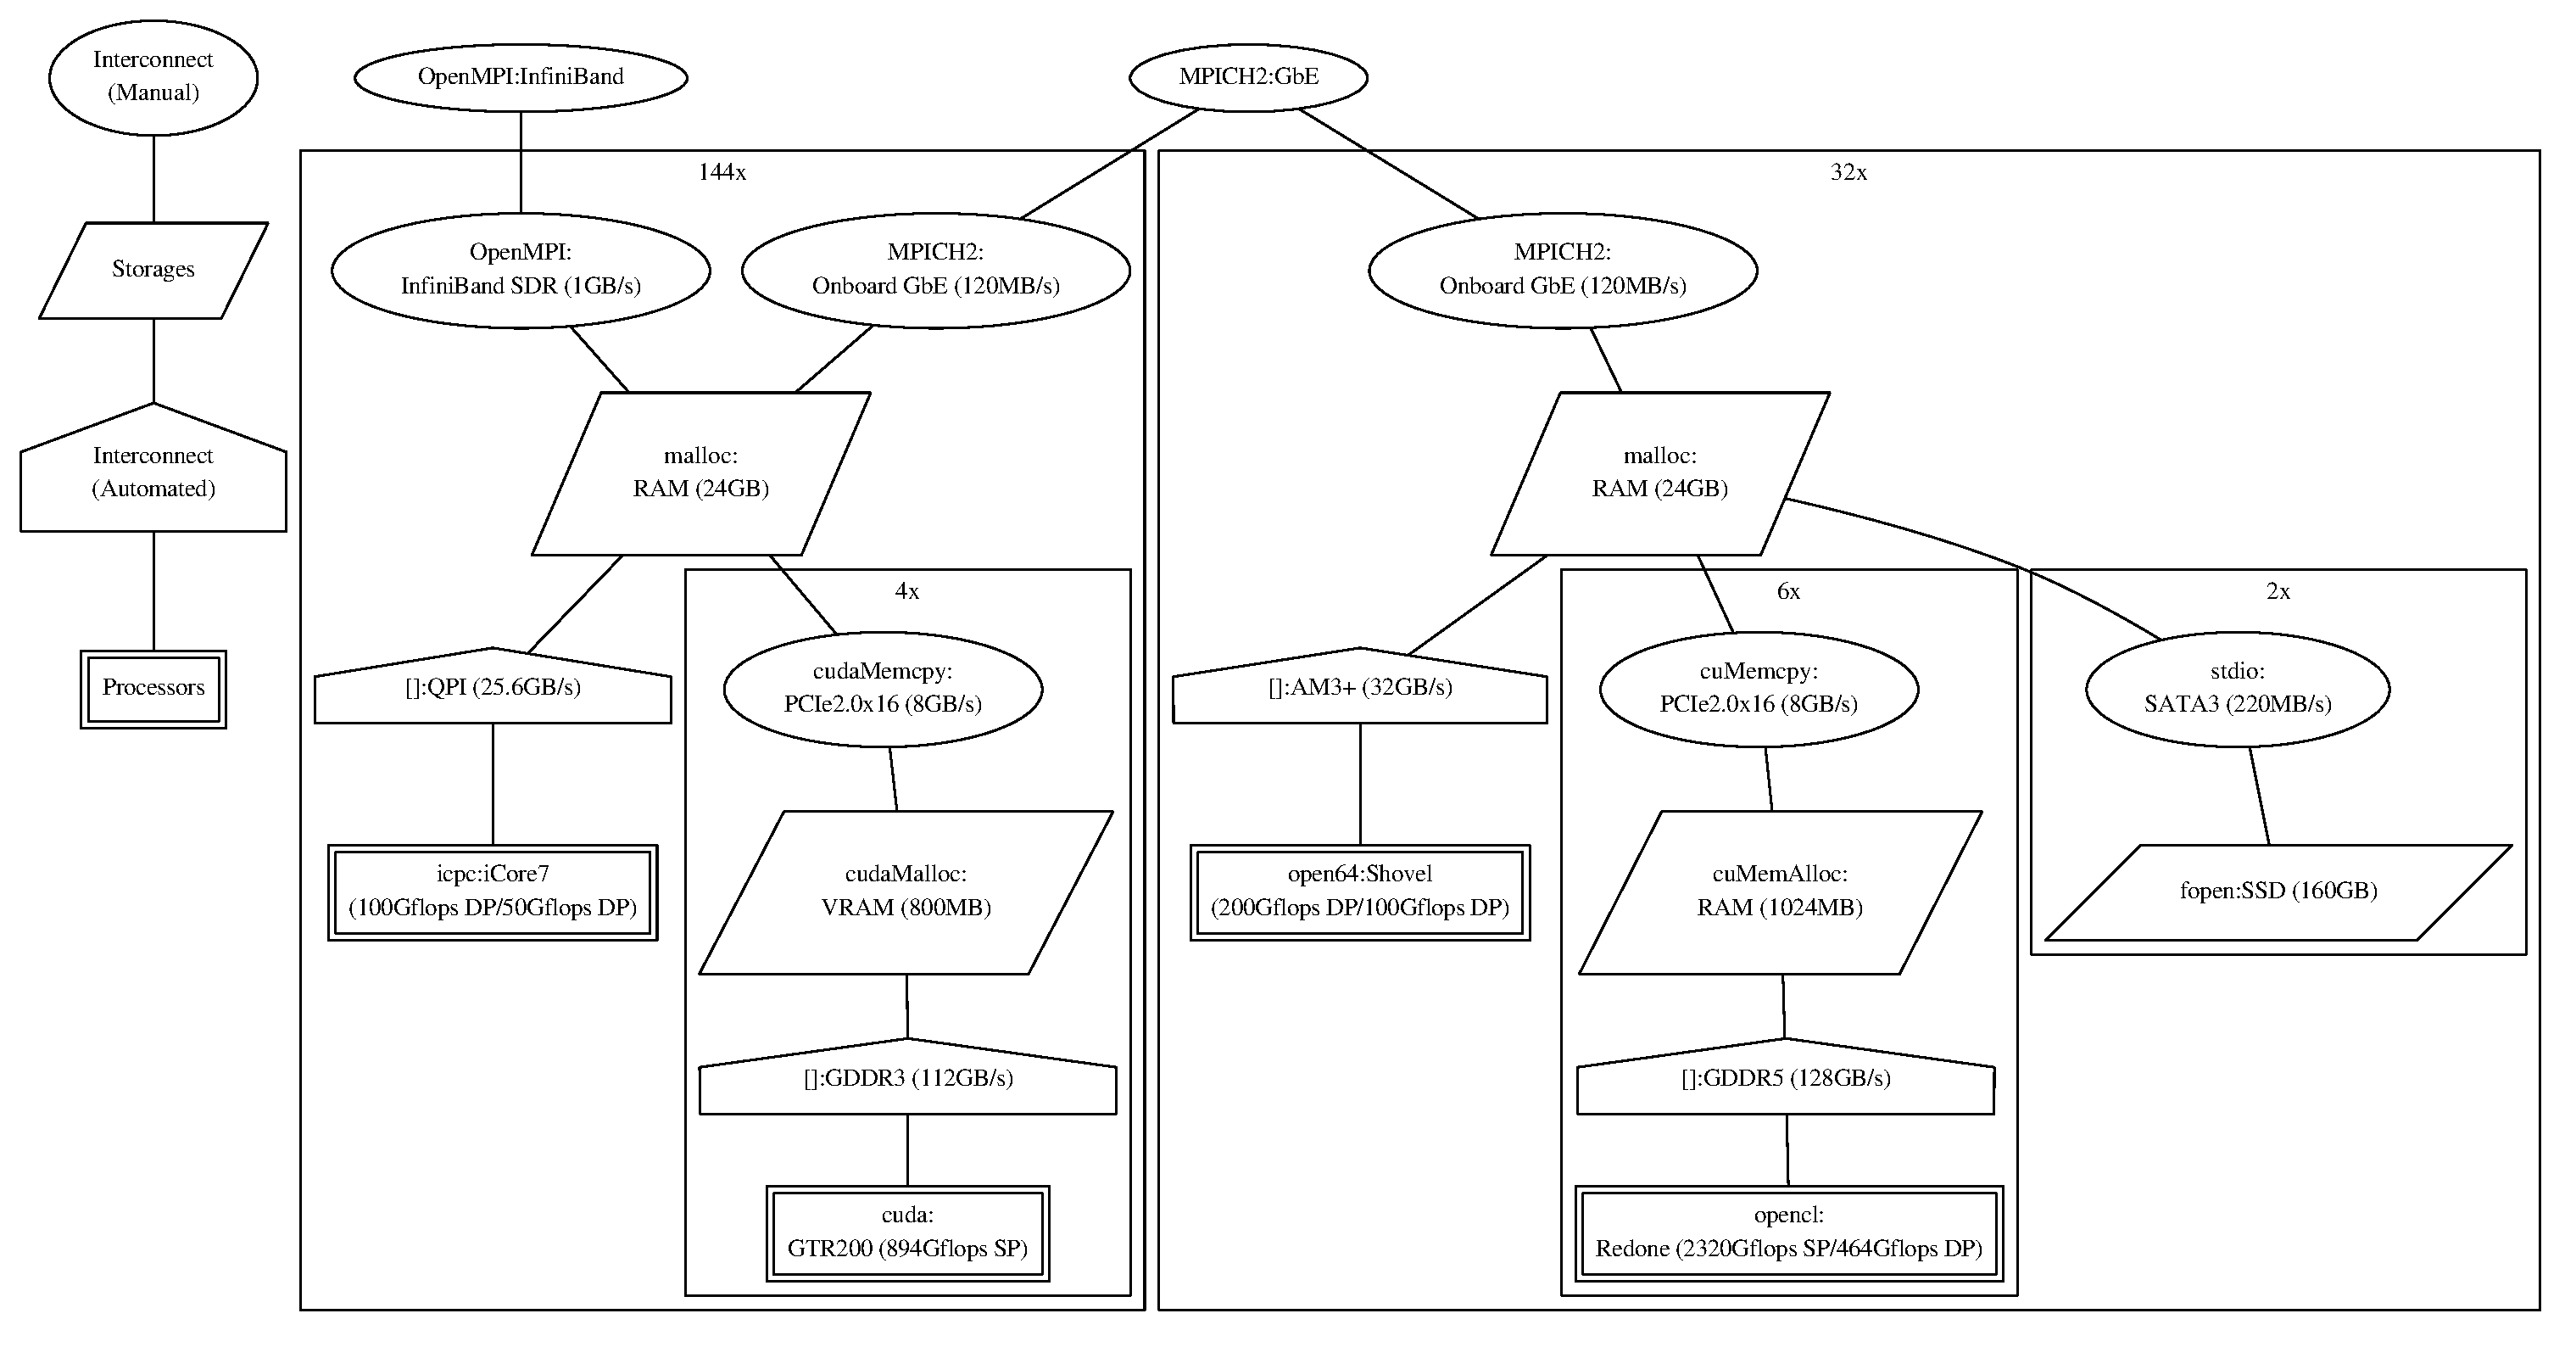
\includegraphics[scale=0.3]{hardware_graph.eps}
  \end{center}
\end{figure*}

\section{Instruction Set}
\subsection{Instruction Set for Primodial Orthotope Machine}
\subsection{Instruction Set for Distributed Orthotope Machine}

\section{Possible Program Transformations}
\subsection{Common Techniques}
A lot of important optimization techniques are known for scalar
processors. Some of them are equally applicable to Orthotope Machine
AST.  Even if we emit the code without such optimizations, we can
expect the native compilers do the job for us. At least Paraiso should
not hinder native optimizations. It's better if we can optimize OM AST
using modern optimization platform such as LLVM.

\paragraph{Constant Folding}
Constant folding is to calculate constant expression in compile
time. It'll be fairly easy, and if we forget to do it, native
compilers are also good at it. One very stupid thing is to store a
globally constant value onto an array. We should avoid this.

\paragraph{Loop Fusion}

{\tt Data.Vector} {\tt Data.Array.Repa}


\paragraph{Common Subexpression Elimination}

To avoid performing the same calculation twice.

\subsection{Timestep Fusion}
\subsection{Cache}
\subsection{Data-Flow-Tree Manipulations by User Specification}
\subsection{Synchronization Insertion}
\subsection{Trapezium Splitting}
\subsection{Parallelogram Splitting}
\subsection{Block Skew}
Fluid consists of multiple orthotope of the same shape.


\bibliography{paraiso}
\end{document}

